\documentclass{llncs}
%
\usepackage{graphicx}
\usepackage{float}
\usepackage{subfigure}
\usepackage{multirow}
\usepackage{makeidx}  % allows for indexgeneration
%
\begin{document}
%
\frontmatter          % for the preliminaries
\renewcommand{\arraystretch}{1.2}
\setlength{\tabcolsep}{10pt}
%
\pagestyle{headings}  
%
\title{Person Enrollment by Face-Gait Fusion\thanks{This work has been supported by the grants P1-1B2012-22 and PREDOC/2012/05 from Universitat Jaume I, PROMETEOII/2014/062 from Generalitat Valenciana, and TIN2013-46522-P from the Spanish Ministerio de Econom\'ia y Competitividad.}}
%Portions of the research in this paper use the CASIA Gait Database collected by Institute of Automation, Chinese Academy of Sciences.
%
\titlerunning{Person Enrollment by Face-Gait Fusion}  

\author{Javier Ortells \and Ram\'on A. Mollineda}

\authorrunning{J.~Ortells et al.} 

\tocauthor{Javier Ortells and Ram\'on A. Mollineda}
%
\institute{Institute of New Imaging Technologies, University Jaume I, Castell\'o, Spain\\
\email{jortells@uji.es, mollined@uji.es}}

\maketitle              

\begin{abstract}
This paper studies the problem of automatic person enrollment based on face-gait fusion within a context of anonymous identification. Enrollment should determine whether an observed subject has been seen before or not. Traditionally, this process has been embedded into a major identification system and its potential has been undervalued. This work claims that enrollment can be considered as a task in itself, and that there are real applications that can benefit from exclusively managing it. To this end, it is shown that the enrollment error model is different from that of anonymous identification. Enrollment experiments, conducted over three types of random permutations of probe samples, showed the benefits of face-gait fusion over single biometrics.

\vspace{-2mm}
\keywords{enrollment, face-gait fusion, anonymous identification.}
\end{abstract}
%
\section{Introduction}\label{sec:introduction}

The anonymous biometric identification problem, as defined in~\cite{DeCann:2012}, consists in assigning a synthetic identity label to a given (\emph{probe}) biometric sample, after comparing it against a number of samples previously collected in a (\emph{gallery}) set. In a conventional approach, a scoring engine computes similarity scores between the probe sample and all gallery samples, and the maximum score is compared with a decision threshold. If this score is above the threshold, a \emph{matching} decision is made and the identity linked to the matched gallery sample is assigned to the probe sample. Otherwise, a \emph{non-matching} occurs, and the probe sample is enrolled in the gallery set under a new synthetic identity dynamically created. Anonymous identification is similar to people re-identification, although the latter is expected also to manage multiple sensors and poses~\cite{Zheng:2011,Roy:2012}.
%,Mogelmose:2013,Matsukawa:2014,Guo:2014}. 

Automatic enrollment has mostly been considered as an indivisible piece of the anonymous identification workflow. That is, both the matching and non-matching events seem to lead to a monolithic response,  where the enrollment decision is embedded. However, by closely examining this process, enrollment can be understood as a more primary decision level than identification. In addition, it is easy to find real applications than can benefit from an enrollment function. The most straightforward one could be to count unique people or, in other words, to strictly address the question ``Has this person been encountered before?''\cite{DeCann:2012}. 

Given a probe sample as input, a basic on-line enrollment approach should determine whether that sample is sufficiently similar to any gallery sample. If so, it is accepted as belonging to a previously \emph{enrolled subject} (no matter who). Otherwise, it is labeled as a \emph{new subject}. In both cases the probe can be added to the gallery set, which could be empty at the very beginning. Note that these class labels 
will depend on the position of the samples in a given sequence: the first sample of someone should be considered as \emph{new subject}, while the rest should be labeled as \emph{enrolled subject} samples. Thus, as in anonymous identification, enrollment efficacy relies heavily on the sequential order of probe samples. 

The main difference of plain enrollment with respect to anonymous identification is that no identities (nor clusters) are required. That is, the gallery can be viewed as a general repository comprising all previously enrolled samples together, without any labeling. Thus, while the number of classes in the anonymous identification problem is a dynamic number that is expected to grow continuously, the enrollment model is based on only two classes. This structural difference may induce different decision rules and error counts, as well as distinct impacts of errors in the future system behavior. In view of the above discussion, this paper is first intended to state that enrollment can be considered as an independent process able to solve interesting problems by itself. 

In this paper, enrollment experiments have been carried out by fusing face and gait scores, which is a popular multi-biometric approach~\cite{Geng:2010,Hossain:2011}. %Behara:2013}
A recent and comprehensive survey can be found in~\cite{Almohammad:2013}. To the best of our knowledge, no automatic enrollment results based on face-gait fusion have been reported in the literature so far. The advantages of combining face and gait rely on the expected complementarity of their properties. While face analysis requires the subject to be close to the sensor, gait can be properly measured in low resolution videos captured at a distance. In addition, frontal faces generally provide more discriminant information than side faces, while the opposite is expected for gait. 

Summarizing, the main contributions of this work are: 1) to state automatic enrollment as a task of interest in itself, by stressing its operational singularities and identifying real applications that capitalize it; and 2) to present, possibly, the first automatic enrollment results from face-gait fusion.

\section{The enrollment problem}

A pure on-line enrollment strategy is intended to determine whether a new probe sample belongs to any known (\emph{enrolled}) subject or 
it is the first occurrence of a \emph{new} subject. A simple operational scope can be defined 
by the following elements:
\begin{itemize}
\item \textbf{Scoring function $s(\cdot)$}. Given a probe sample $p$ and a gallery sample $g$, it computes a match score $s(p,g)$, thus generating a matching hypothesis $h(p,g)$. The function $s(\cdot)$ is usually normalized in $[0,1]$. From now on, it will be assumed that $s(\cdot)$ measures dissimilarity or distance between two samples. 
\item \textbf{Numerical threshold $\gamma$}. A match score $s(p,g)$ is compared with $\gamma$ to make a decision on the acceptance or rejection 
of $h(p,g)$. 
\item \textbf{Gallery set $G$}. It accommodates the samples from the enrollment process. 
\end{itemize}

Given a (probe) sample $p$, the enrollment method searches for the gallery sample $\hat g$ most similar to $p$, and the associated match score $\hat s(p)=s(p,\hat g)$ is used to make a decision. A \textit{matching} takes place if $\hat s(p)\le\gamma$, while a \textit{non-matching} occurs when $\hat s(p)>\gamma$\footnote{Note that the converse holds when scores encode similarities (rather than distances).}. The fact that $\hat s(p)$ omits $\hat g$ means that only the minimum score is required. When the gallery set is empty, $p$ is directly added to $G$.  

Two types of errors are intrinsic to this process:
\begin{itemize}
\item \textbf{False Match} (FM): A matching decision is made, $\hat s(p)\le\gamma$, with $p$ being the first occurrence of a subject, i.e., a sample from the New subject class is misclassified. This FM event also holds in anonymous identification (AI).
\item \textbf{False Non-Match} (FNM): A non-matching decision is made, $\hat s(p)>\gamma$, with $p$ being \emph{not} the first occurrence of a subject, i.e., a sample from the Enrolled subject class is misclassified. This FNM event also holds in AI.
\end{itemize}

Complementarily, two types of hits may occur:
\begin{itemize}
\item \textbf{True Match} (TM): A matching decision is correctly made, $\hat s(p)\le\gamma$, with $p$ being a sample of any previously enrolled subject (no matter who). Note that no condition is imposed on the gallery sample $\hat g$ that supports the decision. That is, $p$ and $\hat g$ could belong to different identities. This TM event does \emph{not} hold in AI, where $\hat s(p)$ is also required to be a genuine score ($p$ and $\hat g$ come from a same identity). Otherwise ($\hat s(p)$ is an impostor score and there exists at least one genuine score), AI designates the event as a FM.
\item \textbf{True Non-Match} (TNM): A non-matching decision is correctly made, $\hat s(p)>\gamma$, with $p$ being the first sample of a subject. It also holds in AI.
\end{itemize}

While anonymous identification assesses a matching decision depending on whether the minimum score is genuine or impostor, plain enrollment analysis is based only on the overall minimum score (disregarding its origin). These two different criteria to judge enrollment hits and misses might lead to distinct true or false event rates, as well as to different optimal threshold values. 

These conjectures were experimentally validated through a simple study. Two enrollment experiments were simulated using the genuine minimum scores (identity-based) and the overall minimum scores (plain), respectively. In the first case, when no genuine score was available, the overall minimum score was used. Optimal thresholds were found as those that lead to the highest geometric mean of enrollment class rates. Average results of optimal thresholds and geometric means, computed over 500 repetitions, are shown in Table~\ref{tab:plainenroll}. This number of trials comes from 100 random permutations of samples of each of 5 independent subsets of people. Face and gait data were extracted from synchronous videos in frontal and side viewpoints\footnote{The reader will find more details on methods and datasets in next sections.}. Results prove that the use of the overall minimum score can lead to different enrollment results, even being slightly better than those obtained by using the genuine minimum score for both biometrics.

%\vspace{-5mm}
\begin{table}[t]
\centering
\begin{tabular}{l|c|c|c|c|}
\cline{2-5}
& \multicolumn{2}{c|}{Identity-based enrollment} & \multicolumn{2}{c|}{Plain enrollment} \\ 
\cline{2-5} 
& Face & Gait & Face & Gait \\ 
\hline
\multicolumn{1}{|l|}{Optimal threshold} & 41,69 & 13,47	& 41,91 & 13,52 \\ 
\hline 
\multicolumn{1}{|l|}{Geometric mean} & 0,946 & 0,974 & 0,948 & 0,975 \\ 
\hline 
\end{tabular} 
\vspace{1mm}
\caption{Identity-based enrollment versus plain enrollment. The second strategy, a much simpler approach, succeeded in solving enrollment without loss of performance.}
\label{tab:plainenroll}
\end{table}

\section{Methodology}\label{sec:methodology}

\vspace{-2mm}
Figure \ref{fig:scheme} depicts a methodology overview. Two classifiers were used as scoring engines: RankSVM~\cite{RaulECCV:2012} and 1-NN. The former has proven to be able to learn from training subjects different to those in the test subset under appearance changes. Meanwhile, 1-NN performs template matching between a probe sample and all gallery samples using the Euclidean distance. Next sections provide details of three other key areas: Face methods, Gait methods and Score fusion. 

\subsection{Data usage}\label{subsec:dusage}

\vspace{-1mm}
Given a dataset containing biometric samples of a number of people, this study randomly separates people into two subsets for training and testing purposes, so that each subject is fully assigned to one of them through all their samples. The Training partition is used to learn some transferable knowledge from subjects different to those who will be enrolled. The Test subset is entirely used as the Probe set, whose samples are gradually added to the Gallery as they occur. 

Three types of random permutations were generated as in~\cite{DeCann:2012}, which are intended to simulate three complexity levels. After randomizing probe people, \emph{Increment Probe} (IP) consists in alternating their samples  strictly following the order given to the people. 
\emph{Random Probe} (RP) arranges probe samples in a purely random order. Finally, after a random permutation of probe people, \emph{Increment Subject} (IS) arranges all probe samples such that all samples corresponding to each particular identity occur in a row. IP (IS) implements the quickest (slowest) way to enroll all people, so it should recreate the easiest (hardest) scenario. RP is expected to lead to in-between situations.

\subsection{Gait methods} 

\begin{figure}[t]
   \centering
   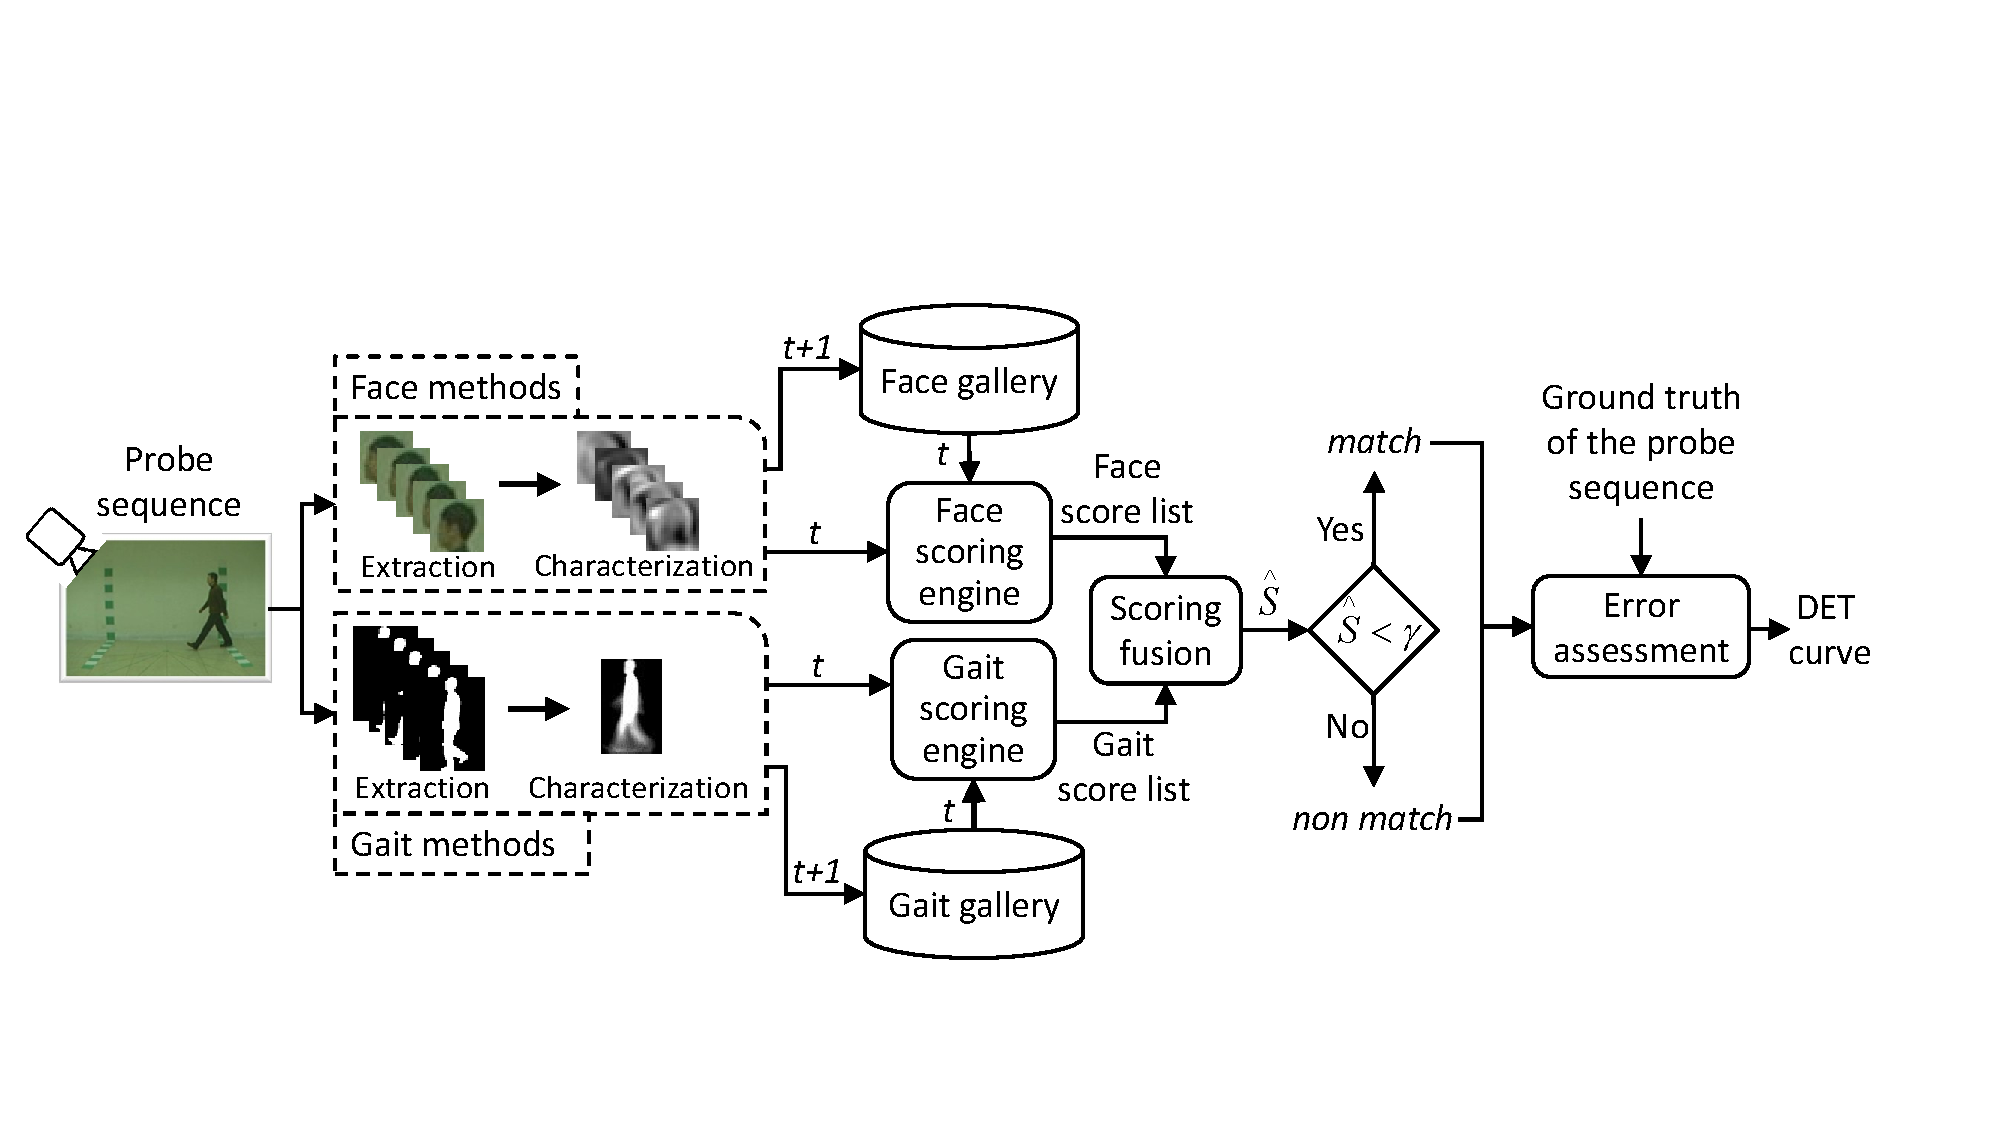
\includegraphics[width=\linewidth]{Figures/scheme.pdf}
   \vspace{-5mm}
   \caption{Methodology overview.}
   \label{fig:scheme}    
   \vspace{-3mm}           
\end{figure}

\vspace{-1mm}
Given a probe video, binary silhouettes from all video frames were extracted, normalized to 44x64 px., and averaged to build a Gait Energy Image (GEI)~\cite{Han2006}. It is a simple but effective model-free characterization method, widely used in gait recognition, which condenses the shape and the dynamics of the body parts.

\subsection{Face methods} 

\vspace{-1mm}
Given a video frame, the face was extracted from the upper 1/7 of the body silhouette area (ROI), as in~\cite{Geng:2010}. Let $w$ and $h$ be the width and the height in pixels of the ROI. ROIs with $h\notin[w/4,3w/4]$ were discarded. Given a suitable ROI, the largest blob contained therein, which is expected to be the face area, was cropped by an $h\times h$ region horizontally centered on the blob's $x$-centroid. Face regions were then converted to gray-scale, histogram equalized and resized to a same resolution ($18\times18$ px. due to database constraints). All pre-processed faces drawn from the frames of a particular video were projected onto the space defined by a Fisherface matrix~\cite{Belhumeur:1997} computed from all available faces in the Training subset. Finally, the projected face images were averaged to build a single face representation of the video under analysis.

\subsection{Face-gait fusion}\label{subsec:fusion}

\vspace{-1mm}

The two biometric scores of a subject are obtained, normalized and combined into a joint score which feeds a threshold-based rule. Given a particular biometric, raw scores are normalized by the $p^{th}$ percentile of the distribution of all \emph{minimum} scores obtained when enrolling an independent subset of training people (one minimum score per sample). Normalized scores above $1$ are truncated at $1$. As each enrollment decision is made solely using the minimum distance, this process is intended to expand differences between minimum genuine scores and impostor ones, so that a suitable threshold can be stated (avoiding the effect of outliers). In this work, $p^{th}$ was set to $90^{th}$. Training people were further divided into two independent subsets, one for learning the RankSVM model and one for estimating the $90^{th}$ score. Given a probe sequence $p$, let ${\hat s}_f(p)$ and ${\hat s}_g(p)$ be the minimum face and gait normalized scores, respectively. The fused score is computed as $s(p)=\alpha\cdot{\hat s}_f(p)+(1-\alpha)\cdot{\hat s}_g(p)$, where $\alpha$ takes value in $\{0,0.25,0.75,1\}$. Note that $\alpha=0$ and $\alpha=1$ represent single-biometric approaches. 

\section{Experiments}\label{sec:experiments}

\vspace{-1mm}
%\subsection{Dataset}
The \textit{Dataset B} of the CASIA gait Database~\cite{Yu:2006} was chosen to assess the proposed methodology, due to its high number of people (124), videos per person (10), and different view angles (11). However, only sequences recorded from 0$^{\circ}$ and 90$^{\circ}$ subject-to-camera angles were considered, as they are supposed to be the most discriminant viewpoints for face and gait description, respectively. The 10 videos per person and angle comprise 6 events under neutral appearance, 2 with changes in clothing and 2 with changes in load carrying. Since all video frames contain the entire body, gait and face data were extracted from them. As a gait database, the resolution was sufficient to build the gait model, but it showed poor to face description. Two experimental studies have been designed:
\begin{description}
\item[Study I: Impact of sample arrangement.] It is intended to probe that enrollment performance strongly depends on sample permutation. To reduce analysis to essentials, face and gait models from \emph{neutral} sequences were separately computed and arranged following the three types of permutations. Results using 1-NN for 0$^{\circ}$ and 90$^{\circ}$ view angles are discussed. 
\item[Study II: Impact of face-gait fusion.] It aims at showing that face-gait fusion leads to better enrollment results than face and gait on their own. %Accordingly,  
RankSVM and 1-NN results based on fusion and on single biometrics were compared using \emph{all} sequences under the RP setting and both viewpoints. 
\end{description}

From each database view regarding angle and appearance filters, 5 independent partitions of people were built as explained in Sect.~\ref{subsec:dusage} and~\ref{subsec:fusion} ($67\%$ Training + $33\%$ Test). Given any of the 5 test subset, 100 sample arrangements were created by chance for each of the three types of permutation. It yielded %a total of 
500 \emph{Detection Error Tradeoff} (DET) curves~\cite{Martin:1997} by experiment, which were finally graphed as a vertically averaged DET curve~\cite{Fawcett2006}. Unlike ROC curves, DET plots FNM rate on the $Y$ axis, focusing on the trade-off between both errors.

\subsection{Study I: Impact of sample arrangement on enrollment}\label{subsec:studyI}

\vspace{-1mm}
\begin{figure}[t]
   \centering
   \subfigure[Side viewpoint (90$^{\circ}$)]{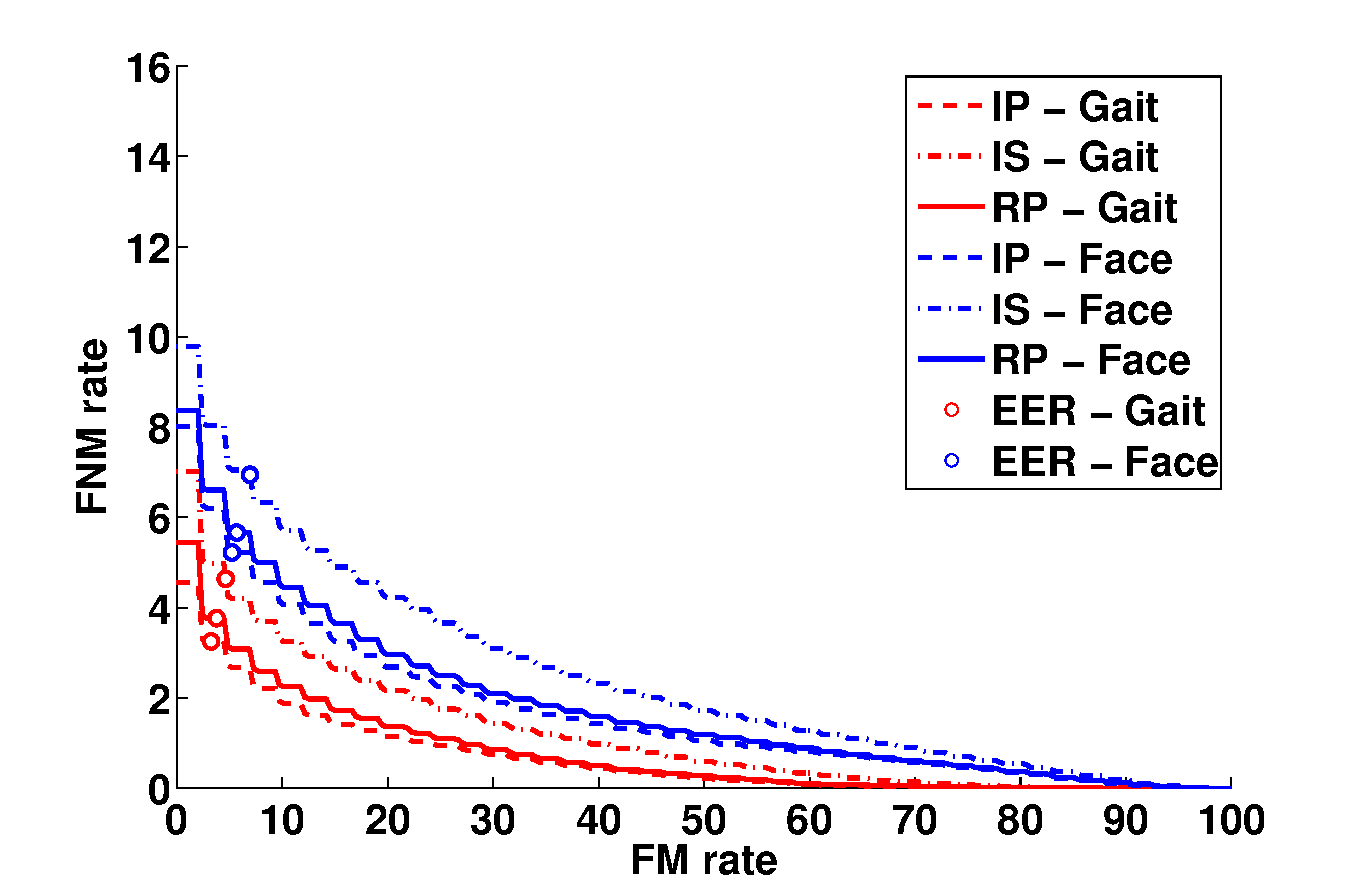
\includegraphics[width=0.495\linewidth]{Figures/Estudio1_090.pdf}\label{fig:studyI:a}} 
   \subfigure[Frontal viewpoint (0$^{\circ}$)]{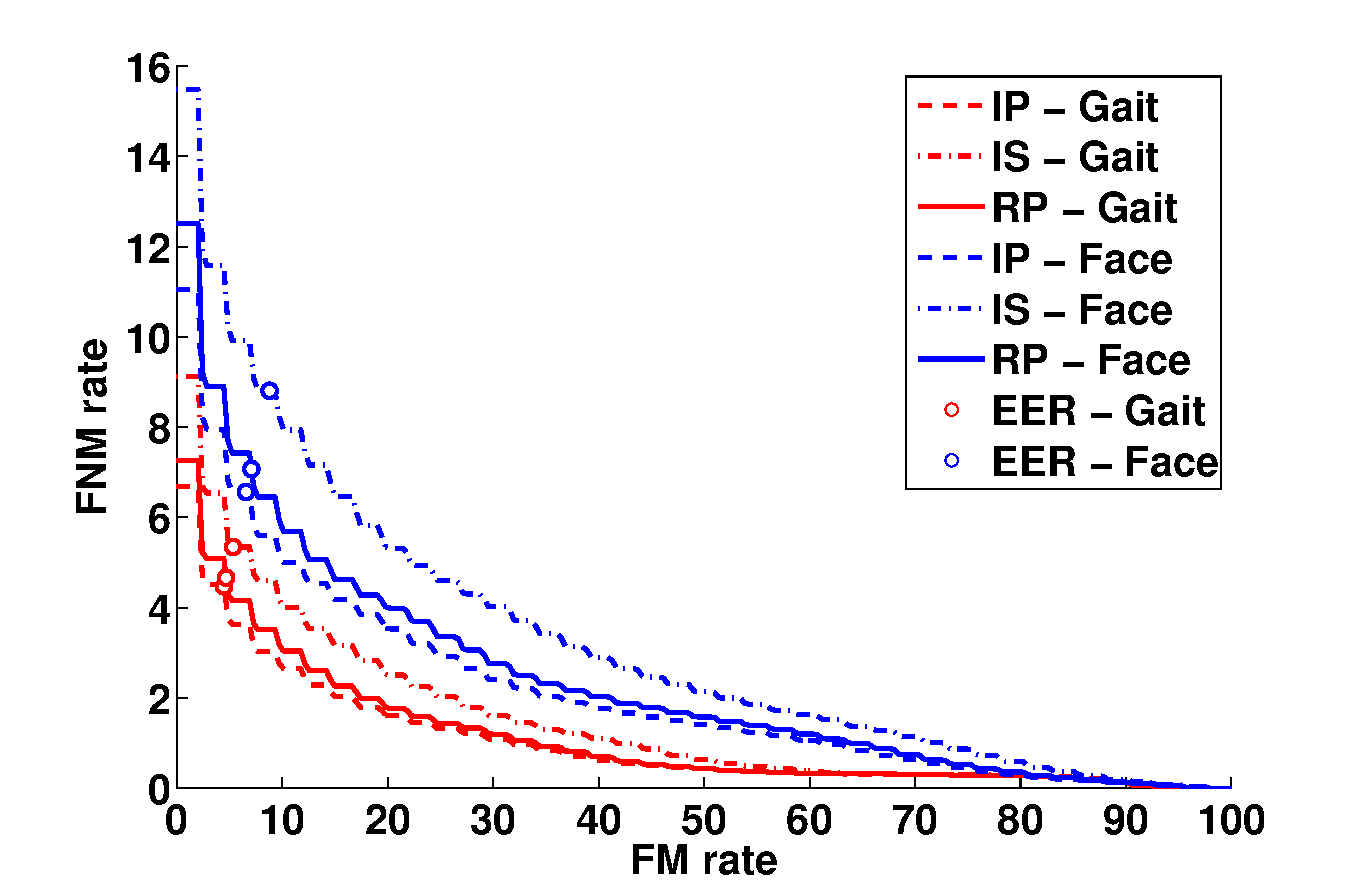
\includegraphics[width=0.495\linewidth]{Figures/Estudio1_000.pdf}\label{fig:studyI:b}}
   \caption{Average DET curves from using 1-NN over \emph{neutral} gait and face samples (without fusion) as regards the three permutation types, both from $0^{\circ}$ and $90^{\circ}$ view angles.}
   \label{fig:studyI}               
\end{figure}

From the analysis of the Fig.~\ref{fig:studyI:a} and~\ref{fig:studyI:b}, two important issues should be discussed. Firstly, gait leads to better enrollment results than those derived from face data for both viewpoints and the three types of permutation. In the case of 90$^{\circ}$ angle, it can be explained by the expected superiority of the side gait over the side face. In the case of the 0$^{\circ}$ angle, the video resolution might be the answer: it seems appropriate for gait description,  but poor for face modeling. Secondly, it has been empirically proved that sample arrangement has a strong impact on enrollment performance. In this regard, the permutation types IP and IS clearly represent the easiest and the hardest scenarios, respectively. This evidence confirms the singularity of pure enrollment, because the effect of both types of arrangement on anonymous identification is just the opposite~\cite{DeCann:2012}.  

\subsection{Study II: Impact of face-gait fusion on enrollment}\label{subsec:studyII}

\vspace{-1mm}
\begin{figure}[t]
   \centering
   \subfigure[1-NN \& Side viewpoint (90$^{\circ}$)]{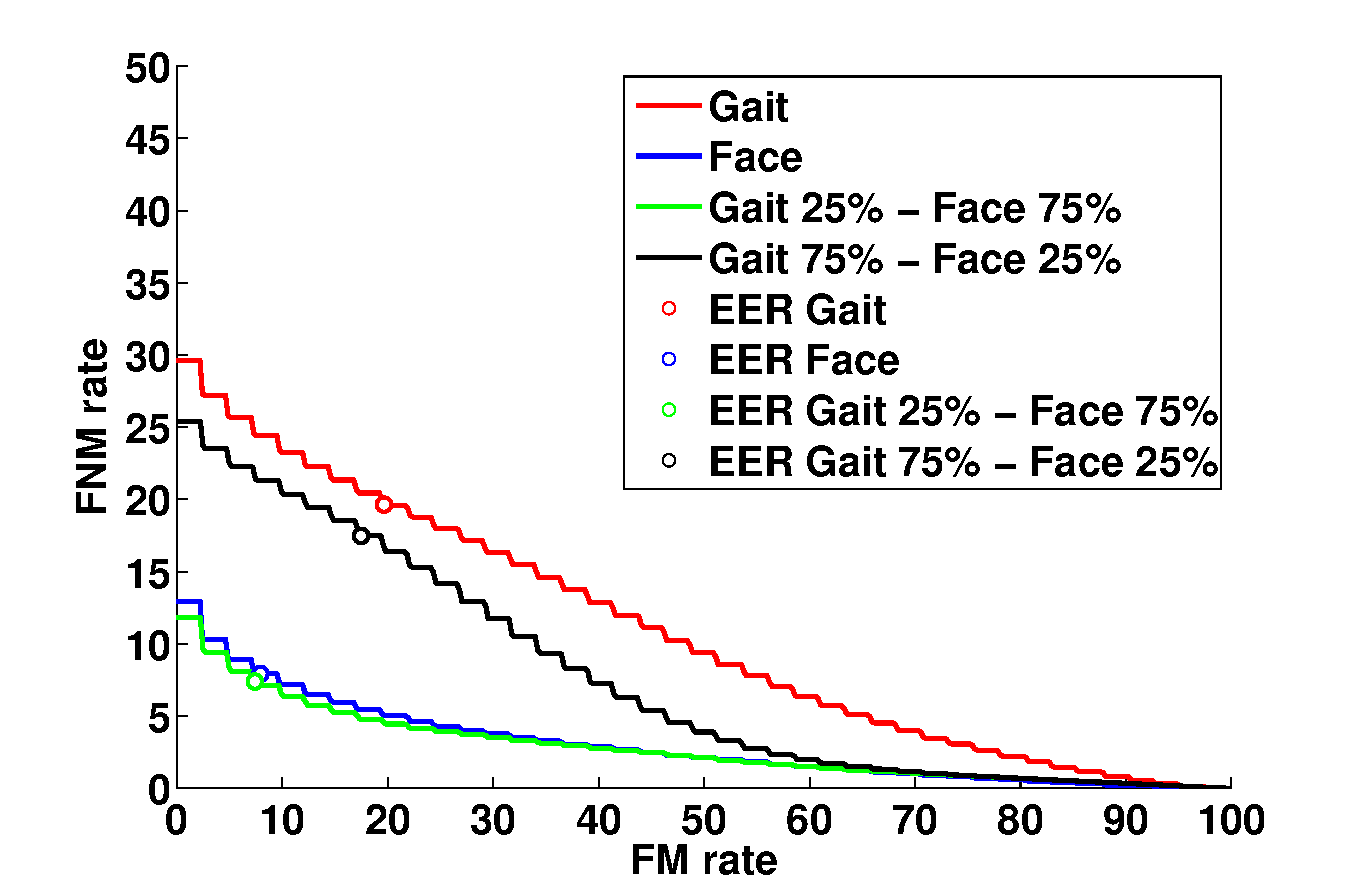
\includegraphics[width=0.495\linewidth]{Figures/Estudio2_1NN_090.pdf}\label{fig:studyII:a}} 
   \subfigure[1-NN \& Frontal viewpoint (0$^{\circ}$)]{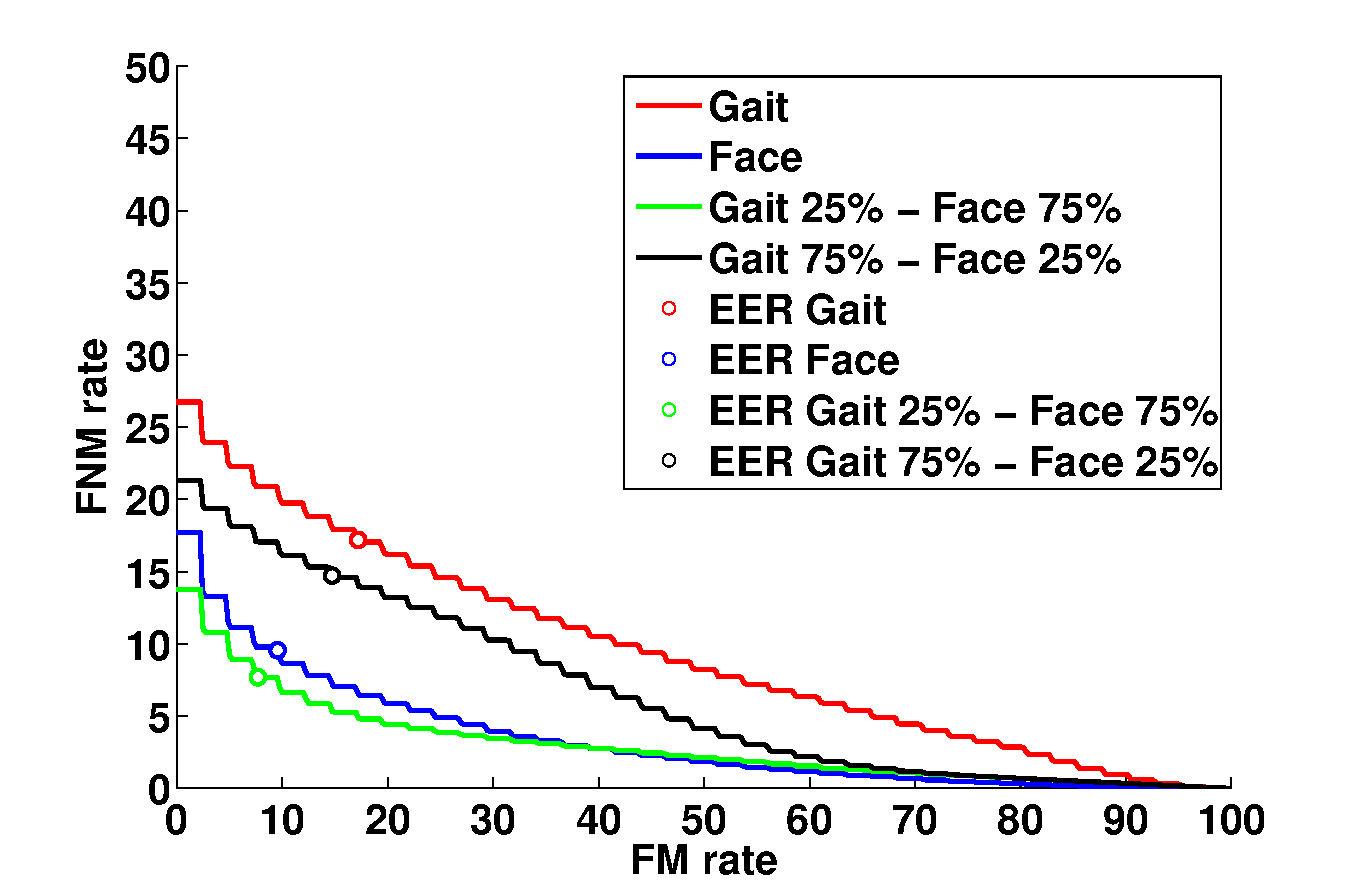
\includegraphics[width=0.495\linewidth]{Figures/Estudio2_1NN_000.pdf}\label{fig:studyII:b}} \\[-1mm]
   \subfigure[RankSVM \& Side viewpoint (90$^{\circ}$)]{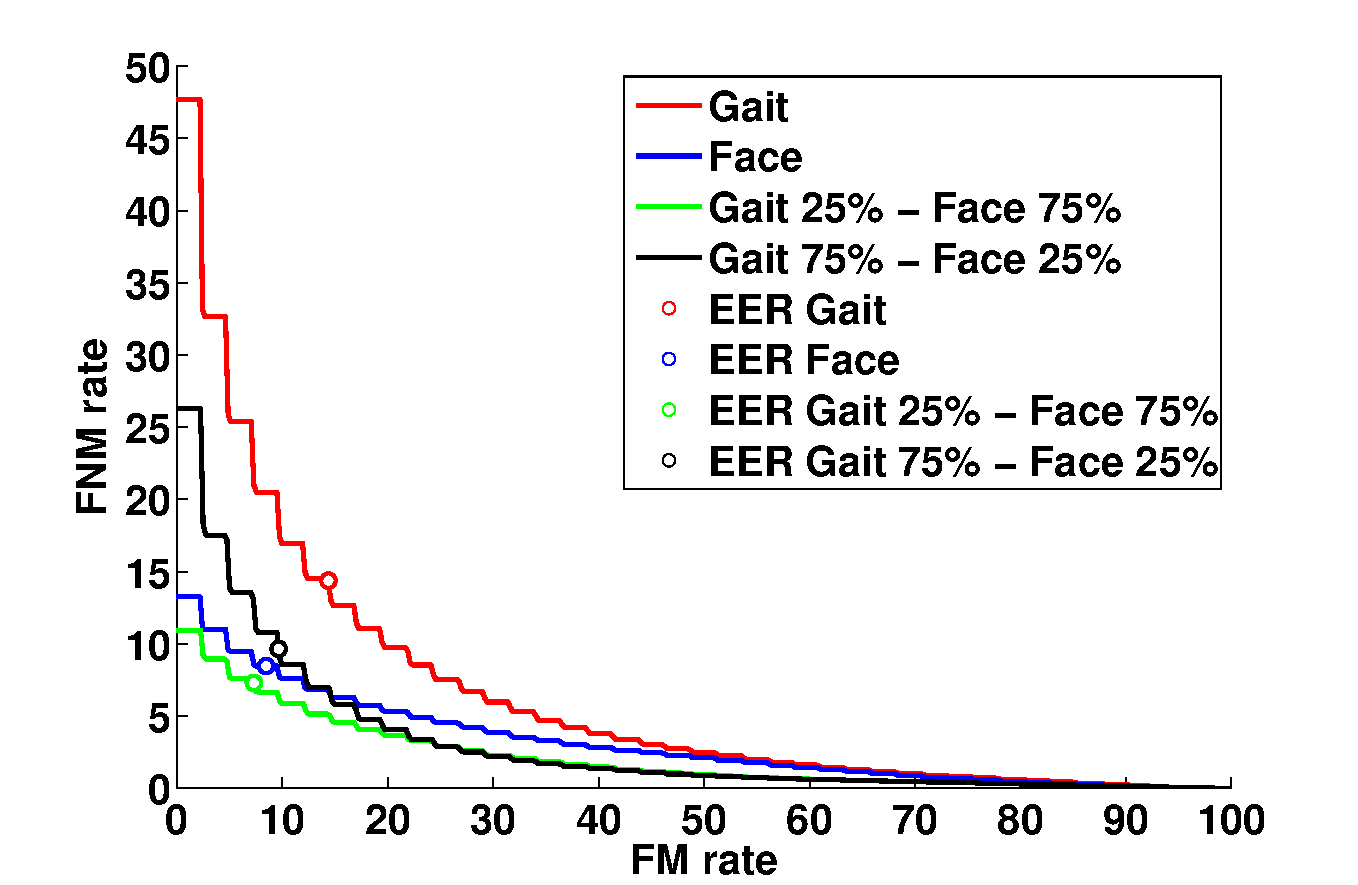
\includegraphics[width=0.495\linewidth]{Figures/Estudio2_RankSVM_090.pdf}\label{fig:studyII:c}} 
   \subfigure[RankSVM \& Frontal viewpoint (0$^{\circ}$)]{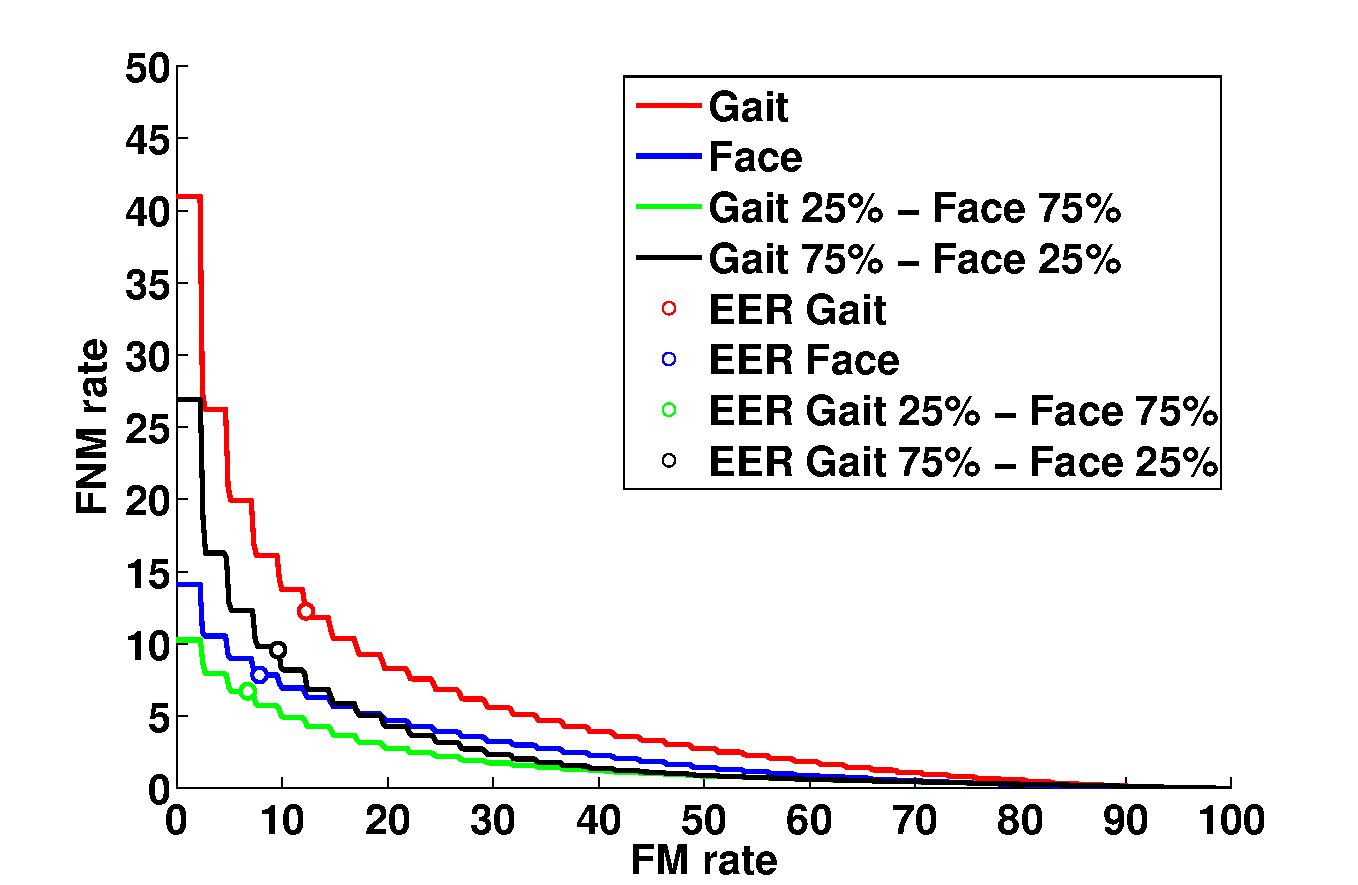
\includegraphics[width=0.495\linewidth]{Figures/Estudio2_RankSVM_000.pdf}\label{fig:studyII:d}}
   \caption{Average DET curves showing 1-NN and RankSVM performances over \emph{all} samples arranged following the RP permutation, both from $0^{\circ}$ and $90^{\circ}$ view angles.}   \label{fig:studyII}               
\end{figure}

In this study, three levels of analysis are worth pointing out: 
\begin{enumerate}
\item \emph{Face vs.~gait}. Unlike the Study I, samples comprise changes in clothing and load carrying. This affects gait appearance more than faces, as shown in Fig.~\ref{fig:studyII:a} and~\ref{fig:studyII:b}. The red and blue solid lines, which depict the gait- and face-based 1-NN behavior on the RP setting (as in Study I), have moved away from the coordinate center as compared to their positions in the Fig.~\ref{fig:studyI:a} and~\ref{fig:studyI:b}, with the gait-based (red) curve being more affected.  
\item \emph{Multi- vs.~single-biometric}. Since results that rely on faces are better than those supported by gait, the fusion scheme that weights more the face-based scores outperformed both single-biometric results in all the experiments.
\item \emph{RankSVM vs.~1-NN}. RankSVM was able to better deal with changes in people appearance than 1-NN. The former led to average fusion \emph{Equal Error Rates} (EER) for both classes of $7.3$ and $6.7$ from $90^{\circ}$ and $0^{\circ}$ respectively, which were slightly lower than the EERs $7.4$ and $7.7$ yielded by 1-NN. 
\end{enumerate}

\subsection{Conclusions}\label{sec:conclusions}

This work is first intended to present automatic enrollment as an independent process able to solve interesting problems by itself. For that purpose, its operational differences with respect to related tasks such as anonymous identification have been identified, as well as real applications that can benefit from exclusively exploiting enrollment. Experiments based on fusing face and gait scores have been conducted, which are possibly the first enrollment research of its kind. A first study was designed to probe that enrollment performance strongly depends on sample permutation. Results showed that the dependency relationship is contrary to that found in anonymous identification. In a second study, the fusion scheme outperformed both single-biometric results in all the experiments.

\bibliographystyle{splncs}
\bibliography{multibiometrics}
\end{document}
